%
% Hoewel wij ons best doen er voor te zorgen dat alles in dit sjabloon
% conform de productspecificatie uit de leertaak is,
% is het uw eigen verantwoordelijkheid om dat te checken.
%
\documentclass{article}

\usepackage{a4wide} % Hierdoor worden de margins van de pagina kleiner
\usepackage{graphicx} % Voor grafische dingen zoals plaatjes
\usepackage{enumerate} % Voor mooiere opsommingen
\usepackage{array} % Voor mooiere tabellen
\usepackage[dutch]{babel} % Om aan te geven dat dit document in het Nederlands geschreven is

\newcommand{\ratvierkant}[5]{% Voor het maken van een rationaliteitsvierkant
\begin{center}
\begin{tabular}{|m{#5}|m{#5}|m{0.4cm}|}
\hline
{\normalfont\upshape Structure} & {\normalfont\upshape Properties} & \\
\hline
{#1} & {#2} & {\normalfont\upshape \rotatebox{-90}{Description~}}\\
\hline
{#3} & {#4} & {\normalfont\upshape \rotatebox{-90}{Physical reality~}}\\
\hline
\end{tabular}
\end{center}
}


\title{Beweren en Bewijzen Leertaak 1}

% Vul hieronder je naam en studentnummer in
\author{Voornaam Achternaam \and Studentnummer}

\begin{document}
\maketitle % Dit commando zet de titel, auteurs en de datum van vandaag op de pagina

% Vul hieronder de antwoorden op de vragen van leertaak 1 in.

\subsection*{Opgave 1}
\begin{enumerate}[a)]
 \item % Je antwoord op vraag 1a
  Als artefact heb ik gekozen\dots  
 \item % Je antwoord op vraag 1b
  Mijn rationaliteitsvierkant:
 
  % Hieronder staat een commando voor het rationaliteitsvierkant.
  % Vervang 'description of structure', 'description of properties',
  % 'thing: an object on physical reality' en 'properties in physical reality'
  % door je eigen antwoorden.
  % De '6cm' kun je veranderen om smallere of juist bredere kolommen
  % te krijgen.
  % Gebruik om een plaatje toe te voegen het volgende commando:
  % \includegraphics[width=0.35\textwidth]{zet hier het pad naar je plaatje, dus alleen naam van plaatje als dit bestand en het plaatje in dezelfde map staan}
 
  \ratvierkant%
  {Amorphous mass of gum}%
  {If it is pressed against softly, it will not move; if it is removed with force, it will fall off}%
  {Piece of chewing gum under the table next to HG00.212}%
  {Put in a mouth and worked with teeth, stuck to the table next to HG00.212, and stiffened}%
  {6cm}

\end{enumerate}

\subsection*{Opgave 2}
\begin{enumerate}[a)]
 \item %2a
  Ik vind de volgende aspecten goed:% Of 'het volgende aspect' als je maar
                                    % 1 ding goed vindt.
  \begin{itemize}
   \item Structure of physical reality, want het onderwerp is duidelijk
   \item Properties of physical reality, want de beschouwde eigenschappen zijn duidelijk
   % Zorg er zelf voor dat hier het juiste aantal \items 
   % komt te staan.
  \end{itemize}

 \item %2b
  Ik vind de volgende aspecten slecht of onduidelijk:
  \begin{itemize}
   \item Description of structure: het is geen beschrijving maar een plaatje
   \item Properties of physical reality: het potlood is niet uit te gummen, maar het spoor van grafiet dat het achterlaat
 \end{itemize}
\end{enumerate}

\subsection*{Opgave 3}
\begin{enumerate}[a)]
 \item %3a
  % Je kunt natuurlijk je schets met Tikz maken en in dit bestand opnemen,
  % maar het is waarschijnlijk makkelijker om met het volgende commando
  % een plaatje in dit document te plakken:
  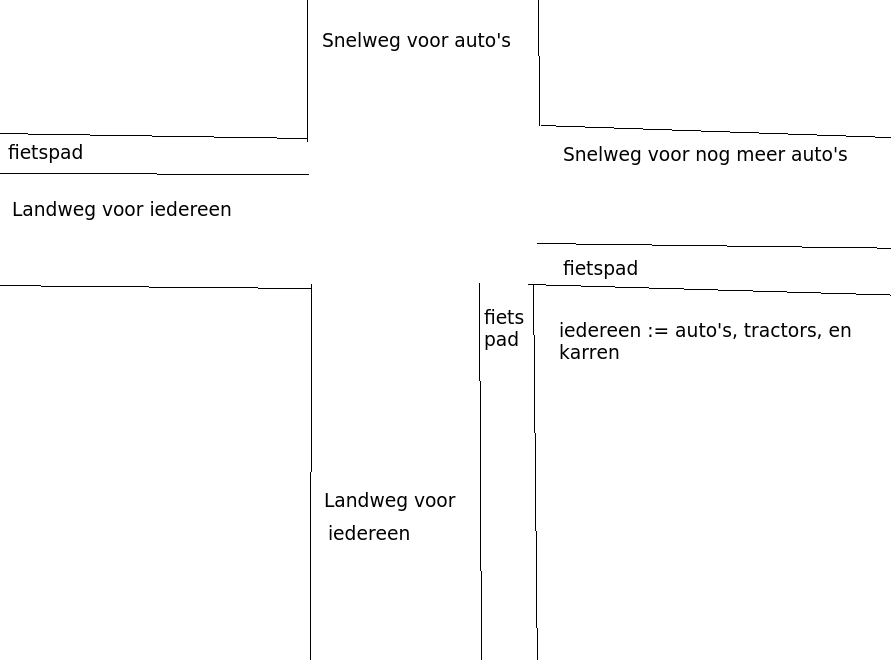
\includegraphics[width=\textwidth]{verkeer.png}


 \item %3b
  Als fietsers naar Marburg willen, mogen ze linksaf, maar dat lijkt me geen goed idee.

 \item %3c
  De informatie op het bord is allemaal nodig op dit moment, want er staat zoveel op dat het handig is om alles twee keer te zien

 \item %3d
  %Dit bord
  %Deze advertentie
  %Deze krantenkop
  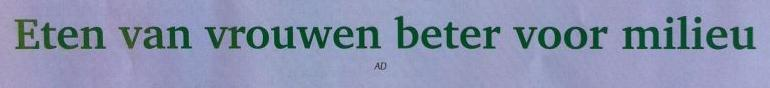
\includegraphics[width=\textwidth]{eerstegoogleresultaatdatiedereeninlevert.jpg}
  
  is mij opgevallen in het kader van onduidelijke beweringen, want "het eten dat vrouwen eten" versus "het opeten van vrouwen".
  % \includegraphics[width=0.35\textwidth]{zet hier het pad naar je plaatje, dus alleen naam van plaatje als dit bestand en het plaatje in dezelfde map staan}
\end{enumerate}
 
\subsection*{Opgave 4}
\begin{enumerate}[a)]
 \item %4a
  Coq gaf bij mij een \dots
  %groen vlaggetje.
  %oranje vlaggetje. Ik denk dat dat komt door\dots
  %rood kruis. Coq heeft moeite met de regel \dots
  
 \item %4b
  De definitie zoals ingevoerd in Coq:
  % verbatim geeft de tekst weer zoals ingevoerd
  \begin{verbatim}
  Definition penguin_logic := 
  \end{verbatim}
\end{enumerate}


\end{document}
